\section{Stellar evolution}
\comment{This section is summarized from \mycitetwo{carroll2007}{ch.12,13,15}}

%use textwidth as width of image
\begin{figure}
  \centering
  \includegraphics[width=\figwidth]{img/molecular_cloud.jpg}
  \caption[Hidden secrets of a massive star-formation region]{
    \label{img:molecular-cloud}
    ``Hidden secrets of a massive star-formation region'' by the Herschel telescope and ESA.
    A giant molecular cloud producing stars when local overdensities in the gas collapses. \\
    Image credit: ESA/Herschel/PACS, SPIRE/Hi-GAL Project. Acknowledgement: UNIMAP / L. Piazzo, La Sapienza – Università di Roma; E. Schisano / G. Li Causi, IAPS/INAF, Italy
  }
\end{figure}


%use \linewidth as fig-width
\begin{figure}
  \centering
  \includegraphics[width=\linewidth]{img/hr_diagram.png}
  \caption[Hertzsprung-Russel diagram]{\label{img:hr-diagram}
    ``The most famous diagram in astronomy is the Hertzsprung-Russell diagram. This diagram is a plot of luminosity (absolute magnitude) against the colour of the stars ranging from the high-temperature blue-white stars on the left side of the diagram to the low temperature red stars on the right side.

This diagram below is a plot of 22000 stars from the Hipparcos Catalogue together with 1000 low-luminosity stars (red and white dwarfs) from the Gliese Catalogue of Nearby Stars. The ordinary hydrogen-burning dwarf stars like the Sun are found in a band running from top-left to bottom-right called the Main Sequence. Giant stars form their own clump on the upper-right side of the diagram. Above them lie the much rarer bright giants and supergiants. At the lower-left is the band of white dwarfs - these are the dead cores of old stars which have no internal energy source and over billions of years slowly cool down towards the bottom-right of the diagram.''
    Image/description credit: Richard Powell [CC BY-SA 2.5] \href{http://www.atlasoftheuniverse.com/hr.html}{atlas of the universe}
  }
\end{figure}

\begin{figure}
  \centering
  \includegraphics[width=\textwidth]{img/various_initial_mass_functions.png}
  \caption{ \label{fig:various-imf}
    A simplified visualization of some of the common initial mass functions in the literature.
    \mycitetwo{cappellari12}{and references therein}, \mycite{salpeter55}, \mycite{kroupa01}, \mycite{chabrier03}, \mycite{miller79}. \\
    image-credit: By JohannesBuchner [CC BY-SA 4.0 (\url{https://creativecommons.org/licenses/by-sa/4.0})], from Wikimedia Commons
  }
\end{figure}

\begin{figure}
  \usetikzlibrary{arrows, positioning, automata}

\newlength{\circleheight}
\setlength{\circleheight}{1.5cm}
\newlength{\circlewidth}
\setlength{\circlewidth}{3.4cm}
\newlength{\horseplength}
\setlength{\horseplength}{8cm}
\newlength{\verseplength}
\setlength{\verseplength}{6cm}

\newcommand{\initialgastext}{\centering \textbf{Interstellar gas} \\ Characterized by initial mass function of stars that will form}
\newcommand{\starformationtext}{\centering \textbf{Star formation} \\ Collapse of initial gas into stars \\ Characterized by the star formation rate}
\newcommand{\stardeathtext}{\centering \textbf{Death of stars} \\ Explosive ejection of enriched gas \\ Characterized by isotopic yield tables}
\newcommand{\inflowtext}{\centering \textbf{Inflow} \\ Prestine gas from extragalactic medium}
\newcommand{\outflowtext}{\centering \textbf{Outflow} \\ Enriched gas ejected from intergalactic medium}

\centering
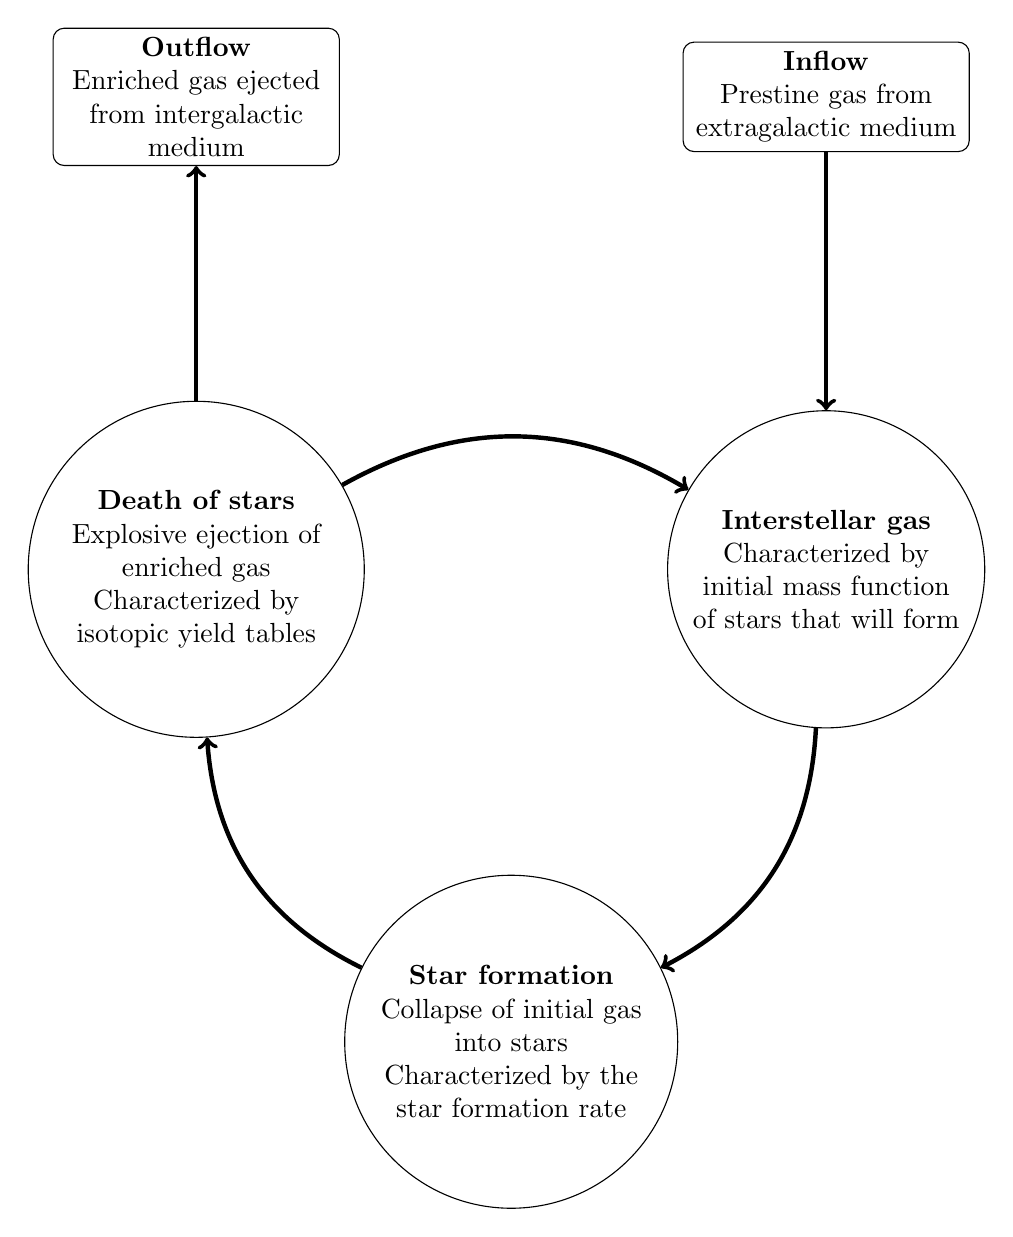
\begin{tikzpicture}[bubble/.style={circle, draw}, flow/.style={rounded corners, draw}]
  %Make nodes with circles of text
  \draw (0.5\horseplength,\verseplength) node[bubble] (A) {\parbox{\circlewidth}{\initialgastext}};
  \draw (0,0) node[bubble] (B) {\parbox{\circlewidth}{\starformationtext}};
  \draw (-0.5\horseplength,\verseplength) node[bubble] (C) {\parbox{\circlewidth}{\stardeathtext}};
  \draw (0.5\horseplength, 2\verseplength) node[flow] (D) {\parbox{\circlewidth}{\inflowtext}};
  \draw (-0.5\horseplength, 2\verseplength) node[flow] (E) {\parbox{\circlewidth}{\outflowtext}};

  %curved arrows between bubbles
  \path (A) edge[bend left, ->, ultra thick] (B);
  \path (B) edge[bend left, ->, ultra thick] (C);
  \path (C) edge[bend left, ->, ultra thick] (A);
  \path (D) edge[->, ultra thick] (A);
  \path (C) edge[->, ultra thick] (E);
\end{tikzpicture}
\caption[Stellar enrichment diagram]{\label{tikz:stellar-enrichment}
  Diagram depicting recycling of gas in a one-zone galaxy model.
  Initially the stellar gas is prestine, from big bang nucleosynthesis, just like the inflow from extragalactic gas.
  Stars form from the prestine gas, forming stellar populations from a given star formation rate and initial mass function.
  Stars end their life asymptotic giant branch stars or explosive type 2 supernovae, ejecting enriched material back into the interstellar medium.
  These events leave remnants, like white dwarves, neutron stars and black holes, which can interact with eachother and other stars to produce secondary explosive events.
  Together the explosive events can drive additional outflow of enriched material away from the galaxy, into the extragalactic medium.
  It should noted that this applies to one-zone models of galaxies, which have two sides; the inside and the outside.
  Ignoring all effects from layered structure of galaxies like; circumgalactic medium, disk, bulge, etc.
}

\end{figure}

Regions of space with higher baryon-density then their surroundings are called giant molecular clouds.
These gas clouds are the birth place of stars\mycitetwo{carroll2007}{ch.12}.
Giant molecular clouds can have masses between $10^3$ and $10^7$ \msol, and extend between a few and a few hundred parsecs \mycitetwo{murray11}{tab.1}.
The same 32 giant molecular clouds observed in \mycite{murray11} is also estimated to contribute to on third of current, total star formation in the Milky Way.
Some regions of these giant molecular clouds will have even larger overdensities and gravity dictates that these overdense regions will eventually fall in on themselves.
A star is a sphere of gas with high enough density, and subsequentally high enough temperature, to maintain stable fusion processes in the core.

\noindent
\begin{minipage}{\textwidth}
  How large such a subregion must be to collapse is given by the Jeans criterion.
  The virial theorem states that for a gas in equilibrium the relation between kinetic energy from thermal motion, $E_k$, and potential energy from gravitational collapse, $E_p$, is given by eq.\ref{eq:virial-theorem}.
  When a cloud of gas collapses, this virial-theorem-equilibrium no longer holds and the gravitational potential energy is greater than the thermodynamical kinetic energy.
  This unequilibrium is called the Jeans criterion\mycitetwo{carroll2007}{ch.12}.

  For a spherically symmetric gas, with no rotation, magnetic fields, turbulence or pressure from outside forces the mass of the subregion must exceed the Jeans mass, eq.\ref{eq:jeans-mass}, or the region must cover a smaller volume then covered by the Jeans radius, eq.\ref{eq:jeans-length}.
  Including an external gas pressure, $P_0$, gives the Bonnor-Ebert mass criterion, eq.\ref{eq:bonnor-ebert-mass}\mycitetwo{carroll2007}{ch.12}.
  
  Assuming that any pressure-gradient inside the gas is too small to affect the dynamics and that all the gravitational potential energy released is effectively radiated away, making the gas isothermal, all parts of the gas will collapse to a single point at the same time\footnote{Naturally the gas can't collapse to a singularity, but it will collapse to a radius very small compared to the original radius.}.
  This kind of collapse is called homologous collapse and the free-fall time when all gas reaches the ``singular point'' is given by eq.\ref{eq:ff-time-collapse}\mycitetwo{carroll2007}{ch.12}.

\end{minipage}
%\hfill
\begin{flushright}
\begin{minipage}{0.75\textwidth}
  \begin{equation}
    \label{eq:virial-theorem}
    2 E_k + E_p = 0
  \end{equation}
  \begin{equation}
    \label{eq:jeans-mass}
    M_J = \left(\frac{5kT}{G\mu m_H}\right)^{3/2}\left(\frac{3}{4\pi \rho_0}\right)^{1/2}
  \end{equation}  
  \begin{equation}
    \label{eq:jeans-length}
    R_J = \left(\frac{15kT}{4\pi G\mu m_H\rho_0}\right)^{1/2}
  \end{equation}
  \begin{equation}
    \label{eq:bonnor-ebert-mass}
    M_{\scriptscriptstyle \textrm{BE}} = \frac{c_{\scriptscriptstyle \textrm{BE}}\left(\frac{kT}{\mu m_H}\right)^2}{P_0^{1/2}G^{3/2}}
  \end{equation}
  \begin{equation}
    \label{eq:ff-time-collapse}
    t_{ff} = \left(\frac{3\pi}{32G\rho_0}\right)^{1/2}
  \end{equation}
  Where $k$ and $T$ is the thermal energy, $G$ is the newtonian gravitational constant, $\mu$ and $m_H$ is the average moleular weight, $\rho_0$ is the initial density of the subregion, $c_{\scriptscriptstyle \textrm{BE}}=1.18$ is a dimensionless constant.
  $E_k$, $E_p$, $M_J$, $R_J$, $M_{\scriptscriptstyle \textrm{BE}}$, $t_{ff}$ are kinetic energy, potential energy, Jeans mass criterion, Jeans length criterion, Bonnor-Ebert mass criterion and free-fall time, respectively
  %% \begin{equation}
  %%   \label{eq:}
  %% \end{equation}
  %% \begin{array}{c}
  %% \end{array}
\end{minipage}
\end{flushright}

When temperatures increase, some of the heavier elements will ionize and the free electrons bonds with hydrogen. The $H^-$ ions increase the opacity drastically trapping the heat from gravitational potential energy more efficiently.
When this happens the collapse will be adiabatic instead of isothermal, and temperatures will increase.
When the gas becomes dominantly adiabatic, but still has no stable fusion process in the core the cloud of gas is called a protostar.
Small fusion processes and increased opacity increases the effective surface temperature and luminosity of the gas cloud\mycitetwo{carroll2007}{ch.12}.

Any inhomogeneities in density, and pressure gradient can cause fracturing of the collapsing gas, as can the presence rotation, turbulence, and magnetic fields.
Fracturing means that the subregion is divided into smaller regions where the density might not be big enough or several protostars can be created.
This might also lead to binary systems or systems with several stars.
The entire giant molecular cloud can also be considered a collapsing gas, but fracturing causes several stars to be born as separate entities inside.

When the density and temperature in the core becomes sufficiently high, the protostar will synthesize hydrogen into helium through the pp-chain, or if the star is massive enough the CNO-cycle.
This period of the stars life is the longest and is called the main sequence.
In the Hertzsprung-Russel diagram (see figure \ref{img:hr-diagram}) this extended curve is well documented, and higher mass stars will find themselves higher in the diagram (more mass means more pressure which means more efficient fusion processes).
Throughout the stars life in the main sequence the luminosity and effective temperature will increase steadily as the overall mean molecular weight changes in the entire star.
The location in the Hertzsprung-Russel diagram (luminosity and surface temperature) when the star first starts to burn steadily (when the star is born so to speak) is called the zero-age main sequence\mycitetwo{carroll2007}{ch.12}

The total time it takes for a gascloud to collapse and reach the zero-age main sequence is inversely proportional to it's mass\mycitetwo{carroll2007}{ch.12}.
The total time of a stars lifetime will depend on it's nuclear timescale, which is roughly, inversely proportional to mass cubed for hydrogen burning\mycitetwo{carroll}{ch.13}.
In short massive stars are quickly born and die more quickly, while smaller stars take alot more time. This makes the smaller stars more susceptible to effects from nearby massive stars that ionize or explode while the smaller stars are still forming.
Dispite this, observations show that the mass distribution function of stars massively favor low mass stars.

\comment{(include plot of initial mass distributions here?)}

\subsection{Nuclear fusion processes}
During the main sequence, where hydrogen is burned into helium in the core, higher mass stars will have a much higher central temperature and density. This means that the hydrogen burning core will be dominated by the CNO-cycle, and the star will have a convective layer that develops in the envelope and stretches deep into the star.
Stars with lower mass will have cores dominated by the pp-chain because their central temperature is lower. The energy transport will also be mostly radiative from the core out to the envelope.
Very low mass stars will develop convective layer from the center outwards.
As the stars age, more hydrogen will burn into helium, and the mean molecular weight will increase, steadily increasing the temperature, radius and luminosity of the stars on the main-sequence\mycitetwo{carroll}{ch.13}.
\comment{Add ranges of solar masses to the different types of stars}

When the core of a low-mass star is depleted of hydrogen and filled with helium the pp-chain will stop in the core, but it will continue in a shell around the core due to high temperatures. The hydrogen burning shell around the core will provide more energy and cause the envelope to expand, this causes the luminosity to increase, but surface temperature to decrease.
higher mass stars will contract, and the convective layer disappears steadily as the core runs out of hydrogen fuel. The contraction heats the core and hydrogen shell burning will power the star\mycitetwo{carroll}{ch.13}.

More and more helium is accreted onto the inert, isothermal helium core, which will collapse when it reaches the chandrasekhar limit.
The collapse of the core causes heating, which inflates the envelope.
Inflating the envelope causes the surface temperature to decrease, this is called the sub giant branch.
The inflated envelope stabilizes and becomes convective from the large temperature gradient.
The effective energy transport causes the luminosity to increase, and the star moves into the red giant tip.
This leads to the first dredge-up where material from outside the core can be mixed into the upper envelope.
The collapsed core can now start fusing helium into carbon and oxygen through the triple alpha process.
The core will then expand, cooling the hydrogen shell and decrease the overall luminosity of the star. Stars with lower masses will develop a electron degenerate core which will cause the core helium flash once the helium is ``ignited'' nearly simountaneously\mycitetwo{carroll}{ch.13}.

The envelope will contract following the expansion of the helium burning core, causing the effective surface temperature to rise. When stable radius, helium burning core and hydrogen burning shell is reached the star will have settled onto the horizontal branch. This is the main sequence equivalent of helium burning stars. As the helium is exhausted in the core, the core will start to contract, expanding the envelope, and the effective surface temperature will decrease toward the redder side of the horizontal branch\mycitetwo{carroll}{ch.13}.

When the heliumn has been expended in the core, it leaves an inert core of carbon and oxygen with a helium burning shell around it.
The helium burning shell will dominate over the hydrogen burning shell lying on top of it and the increased temperature will cause the hydrogen burning shell to expand.
The decreased density of the hydrogen burning shell lowers nuclear reaction rates.
When the helium burning shell exhausts all it's fuel the envelope will expand and become convective, the ensuing mix of material, from the bottom envelope (helium burning shell) to top envelope is called the second dredge-up.
The convective energy transport is more effective, increasing the luminosity of the star.
In the Hertzsprung-Russel diagram, this moves the star up into the asymptotic giant branch.
At this point, the hydrogen burning shell will dominate the energy production of the star once again.
\comment{order of magnitude estimates}
The ``ash'' from the hydrogen burning shell (the top shell) will ``rain'' down onto the inert helium burning shell (bottom shell).
When the temperature is high enough and the bottom shell has enough material, the bottom shell of helium will ignite.
Due to the isothermal layer of the helium shell, triple alpha burning will commence in the entire shell simountaneously, in an explosive fashion.
This explosion, called the helium shell flash, is less explosive the the helium core flash, but might eject more material because it is closer to the surface.
When the helium has been exhausted once again, the shell compresses and the entire process repeats. The repetition of helium flashes is called the third dredge-up, mixing material from the hydrogen and helium shells into the upper envelope\mycitetwo{carroll}{ch.13}.

During the asymptotic giant branch stars loose alot of their material by ejection into the interstellar medium. e.g. from helium flashes, pulsations of the envelope, high luminosity, low surface gravity, high radiation pressure.
The combination of effects is not surely determined, but simulations and observations show that the mass-loss must be great during this stage\comment{ref to sims/obs paper}.

After the helium-flashes have subsided, the envelope has been ejected, and the shell-burning have stopped, the star remains as a hot inert core of carbon and oxygen (with some hydrogen and helium surrounding it). This remnant is called a white dwarf.
This white dwarf will continue to glow until it has radiated away all it's thermal energy\mycitetwo{carroll}{ch.13}.

\subsection{Evolution of massive stars}
While less massive stars $M \lesssim 8 \msol$ become white dwarves, stars with mass $M \gtrsim 8 \msol$ evolve a bit differently.
They have no helium flashes.
Their high mass means that the central density, pressure, and temperature will be higher.
The hydrogen burning core will fill up with helium, and when sufficient mass has been reached, the helium will start to fuse into carbon and oxygen through the triple alpha process and hydrogen will burn in a shell around it.
The carbon in the core will then continue to fuse with more helium into oxygen and neon, with some sodium and magnesium produced.
The oxygen in the core will eventually start to fuse into silicon, and the silicon will eventually start to fuse into sulfur, argon and iron.
In this high temperature and high density environment, this process will not be straight forward, many different carbon isotopes will fuse with other particles into many different heavier isotopes. The details above outlines the general trend.
Assuming that there is an equilibrium of nuclear reactions, the stellar interior will resemble an onion-like shell structure with the heaviest elements deepest in the star\mycitetwo{carroll}{ch.15}.

Fusion processes cannot produce excess energy for elements heavier than iron, although trace amounts of heavier elements can be created from the excess thermal energy.
In the centre of the core, the free electrons can merge with the free protons to create neutrons and release neutrinos
\comment{add nuclear reactions}
The sudden loss of electrons causes the electron degeneracy to drop suddenly and the centre of the core will collapse supersonically until the density is roughly 3 times the nucleon density.
At this point the centre of the core, consisting of mostly neutrons will experience a repulsive effect of the strong nuclear force.
This is equivalent to a Pauli exclusion principle of neutrons.
The repulsive force causes the core to stiffen and rebound. The shock from the rebounding core meets the falling core on top, causing a shockwave that travels outward from the inner core.

Simulations suggest that the shockwave released will be absorbed by the surrounding layers.
The stalled shockwave leaves a shell of high density behind.
This shell is dense enough to absorb a significant amount of the neutrinos released during collapse.
If a small amount of the neutrino energy is transferred to the stalled shockwave it will restart and eject the surrounding layers into the interstellar medium.
The travelling shockwave can be observed as a type Ib, Ic, or II supernova, also called a core collapse supernova.
The remnant of such an event will be a neutron star or (if the mass is great enough to overcome the repulsive force of the strong nuclear force) a black hole\mycitetwo{carroll}{ch.15}.
\comment{Mass limits of black hole/neutron star, both core and initial mass limits}

\subsection{Type 1a supernova}
Star systems can be both single and binary, a study by \mycite{lada06} estimates that 1/3 of all star systems are binary.
``When a white dwarf (WD) composed of carbon and oxygen accreting mass from a companion star in
a binary system approaches the Chandrasekhar mass [$M_{Ch} \simeq 1.38$ solar masses (\msol)], high temperature
causes the ignition of explosive nuclear burning reactions that process stellar material and produce energy.
The star explodes leaving no remnant, producing a Type Ia supernova (SNIa) (K. Nomoto, F.-K. Thielemann, K. Yokoi, ApJ 286, 644 (1984)).''\mycite{mazzali07}

In the thermonuclear explosion iron peak elements (mostly Ni and Fe isotopes and below) are synthesized and ejected into the interstellar medium.
During accretion, helium and hydrogen burning layers develop and helium flashes occur.
These flashes can cause major mixing of hydrogen into the carbon-layers which again can cause neutron-producing reactions in greater numbers.
Neutron capture processes can occur on the surface of type 1a supernovae if the produced neutron densities are high enough (\mycite{nomoto84}).
The isotope distributions also seemed to fill in some missing yields from type II supernovae.

Typical type 1a supernovae are heated from the deacy of \isotope{56}{28}{Ni} and will eject $\simeq 1.4 \msol$ of material at a ejecta velocity of $\simeq10 Mm s^{-1} \simeq 0.03c$ (\mycite{tanaka16}).

\subsection{Neutron star mergers}
The idea of mergers of compact objects (either neutron stars or black holes) by emission of gravitational waves have been around for a long time. Since these events are rich in neutrons, they have been suggested as a potential site for r-process nucleosynthesis
(\comment{ref BBFH? ref something}).
This makes makes neutron stars particularly intersesting for the problem in this thesis \comment{rewrite?}
The general concept is build on two compact objects orbiting eachother, interacting with the spatial curvature and creating ripples.
These ripples maifest as waves in the fabric of space-time and carry gravitational energy away.
The two objects move closer as a result of the energy-loss, and increases the orbital velocity accordingly (\mycite{tanaka16}).
These gravitational waves distort space itself and can be detected by large laser interferometers that detect spatial disturbances smaller then the width of a nucleus (\mycite{abott16}).

The material ejected from a binary neutron star merger, or a kilonova, is heated from the decay of r-process elements.
The mass and velocity of the material is debated,
but estimates are around $v=30-60 Mms^{-1} = 0.1-0.2c \quad m \simeq 0.01 \msol$ (\mycite{tanaka16}).

During a neutron star merger, the two stars move closer to eachother over time from gravitational radiation. When they are close enough to eachother they will disrupt each others surface, and surround the merging bodies in a cloud of neutron heavy material that is ejected into the interstellar medium.
The forces that pull apart the neutron stars surface is only gravitational pull and centripetal force.
As the main bodies merge, a shock drives ejection of material that will bombard the surrounding cloud.
As the envelope expands from the colliding stars, the density of neutronmatter will drop until extremely neutron-heavy nuclei will form, like droplets from steam.
These nuclei are unstable and will \betadecay to more stable isobars.
These heavy nuclei will act as seeds for the neutronrich shockwave emitting from the collision.
\comment{find proper ref on where seeds come from}
The stream of very dense, high-velocity neutrons onto seed of heavy nuclei is the perfect recipe for r-process nucleosynthesis\mycite{tanaka16}.

\subsection{Debate over site of r-process nucleosynthesis}
The exact astrophysical site which dominates the r-process production in the galaxy have been greatly debated over the years.
The main goal in searching for these sites have been to reproduce the peaks in r-process abundance.

At first believed to be caused from shock and neutrino wind during core collapse supernovae, simulations have difficulty reproducing the required conditions (\mycite{thielemann11}).
The two main problems with neutrino driven wind supernovae are high entropies and cannot accurately reproduce the r-process abundance below (A<120) the second r-process peak (\mycite{thielemann11}).
Three-dimensional hydrodynamical simulations have lead to some cases of bipolar ejection of jets (\mycite{winteler12}), and this have been shown to reproduce the second and third r-process peaks.

Initially suggested by \mycite{latrimer74} the tidal disruption of a neutron star can create r-process elements, and in great quantities.
Mergers from gravitational radiation between black holes and neutron stars, or two neutron stars are rare, however the results \mycite{rosswog00} suggest that the amount of r-process material ejected per event makes up for the rarity of events.
Simulations from \mycite{freiburghaus99} also show that, depending on the electron fraction and equation of state used, neutron star mergers eject material with solar r-process abundance between the second and third r-process peak.
A model of ejecta envelope from two merging neutron stars is presented in \mycite{li98}.
They find that the luminosity curve (after making simplifying assumptions) would peak at $L \simeq 10^{44} erg s^{-1}$.
This is similar to a bright supernova, but will last alot shorter (roughly a day).
